% Explanatory overview of our current ideas on learning local structure and motion.
% Written for a first-time reader: what each part does, and why it is there.
% Compile twice with pdflatex. No external files are required.
\documentclass[11pt,a4paper]{article}
\usepackage[T1]{fontenc}
\usepackage[utf8]{inputenc}
\usepackage{lmodern}
\usepackage[margin=24mm,headheight=14pt]{geometry}
\usepackage{amsmath,amssymb,mathtools}
\usepackage{booktabs,tabularx,array}
\usepackage{microtype}
\usepackage{fancyhdr}
\usepackage{enumitem}
\usepackage[hidelinks]{hyperref}
\hypersetup{pdftitle={Learning Local Structure and Motion from Simulation: what we do, how, and why},pdfauthor={},pdfsubject={Overview of current ideas}}
\numberwithin{equation}{section}
\newcommand{\R}{\mathbb R}
\newcommand{\sm}{\mathrm{sm}}
\newcommand{\enc}{\mathrm{enc}}
\setlength{\parindent}{0pt}
\setlength{\parskip}{0.35em}
\setlength{\emergencystretch}{2.5em}
\setlist{itemsep=2pt,topsep=3pt,parsep=0pt}
\pagestyle{fancy}\fancyhf{}
\fancyhead[L]{\small Learning local structure and motion: what we do, how, and why}
\fancyfoot[C]{\small\thepage}
\renewcommand{\headrulewidth}{0.3pt}
\widowpenalty=10000\clubpenalty=10000
\title{\vspace{-1.5em}\Large\bfseries Learning Local Structure and Motion from Simulation\\[5pt]
  \large\mdseries What we do, how, and why}
\author{}\date{}

% Editable TikZ diagrams; no external image files are used.
\usepackage{tikz}
\usetikzlibrary{arrows.meta,calc,positioning,decorations.pathreplacing}
\usepackage[font=small,labelfont=bf]{caption}
% Shared figure typography and restrained print palette.
\definecolor{pcmInk}{HTML}{242424}
\definecolor{pcmBlue}{HTML}{315E8A}
\definecolor{pcmGreen}{HTML}{287668}
\definecolor{pcmAmber}{HTML}{9B632D}
\definecolor{pcmGray}{HTML}{505050}
\definecolor{pcmRule}{HTML}{A0A0A0}
\tikzset{
  pcm/base/.style={rectangle,line width=.4pt,
    align=center,inner xsep=4pt,inner ysep=5pt,outer sep=1pt,
    font=\rmfamily\fontsize{10}{12.4}\selectfont,
    text=pcmInk,execute at begin node={\hyphenpenalty=10000\exhyphenpenalty=10000}},
  pcm/model/.style={pcm/base,draw=pcmBlue!75,fill=pcmBlue!3},
  pcm/physical/.style={pcm/base,draw=pcmGreen!75,fill=pcmGreen!3},
  pcm/text/.style={align=center,inner sep=0pt,text=pcmInk,
    font=\rmfamily\fontsize{10}{12.4}\selectfont},
  pcm/small/.style={pcm/text,font=\rmfamily\fontsize{9.4}{11.6}\selectfont},
  pcm/tiny/.style={pcm/text,font=\rmfamily\fontsize{8.6}{10.4}\selectfont},
  pcm/head/.style={anchor=west,inner sep=0pt,text=pcmInk,
    font=\rmfamily\bfseries\fontsize{10.4}{12.4}\selectfont},
  pcm/arrow/.style={-{Latex[length=1.6mm,width=1.2mm]},line width=.5pt,draw=pcmGray},
  pcm/bluearrow/.style={pcm/arrow,draw=pcmBlue},
  pcm/greenarrow/.style={pcm/arrow,draw=pcmGreen},
  pcm/amberarrow/.style={pcm/arrow,draw=pcmAmber},
  pcm/brace/.style={decorate,decoration={brace,amplitude=4pt},line width=.4pt}
}
\newsavebox{\pcmFigureBox}
\newcommand{\PlacePCMDiagram}[1]{%
  \sbox{\pcmFigureBox}{#1}%
  \typeout{PCM-DIAGRAM width=\the\wd\pcmFigureBox; height=\the\ht\pcmFigureBox; linewidth=\the\linewidth}%
  \ifdim\wd\pcmFigureBox>\linewidth
    \PackageError{pcmfigures}{Diagram exceeds text width}{Reduce diagram geometry, not the document margins.}%
  \fi
  \usebox{\pcmFigureBox}%
}
\setlength{\textfloatsep}{15pt plus 2pt minus 2pt}
\setlength{\intextsep}{15pt plus 2pt minus 2pt}

% Shaded "why" boxes: a short argument set apart from the description.
% The content is collected in a vertical box and split at page breaks, so a long
% box continues on the next page instead of leaving a gap.
\makeatletter
\newbox\pcmWhyAll
\newbox\pcmWhyPart
\newdimen\pcmWhyAvail
\newcommand{\pcmWhyPiece}[1]{%
  \noindent\hbox{{\color{pcmAmber}\vrule width 1.6pt}%
    \setlength{\fboxsep}{7pt}\colorbox{pcmAmber!5}{\vbox{\unvbox#1}}}\par}
\newcommand{\pcmWhyEmit}{%
  % A split piece is re-boxed at its natural height, so stretch reports do not apply.
  \vbadness=10000
  \loop
    \par
    \ifdim\pagegoal=\maxdimen
      \pcmWhyAvail=\dimexpr\vsize-14pt\relax
    \else
      \pcmWhyAvail=\dimexpr\pagegoal-\pagetotal-19pt\relax
    \fi
    \ifdim\dimexpr\ht\pcmWhyAll+\dp\pcmWhyAll\relax>\pcmWhyAvail
      \ifdim\pcmWhyAvail<3\baselineskip
        \newpage
      \else
        \setbox\pcmWhyPart\vsplit\pcmWhyAll to \pcmWhyAvail
        \pcmWhyPiece\pcmWhyPart
      \fi
    \else
      \pcmWhyPiece\pcmWhyAll
    \fi
  \ifvoid\pcmWhyAll\else\repeat}
\newenvironment{why}[1][Why]{%
  \par\addvspace{.55em}%
  \setbox\pcmWhyAll\vbox\bgroup
    \hsize=\dimexpr\linewidth-1.6pt-14pt\relax
    \@parboxrestore\fussy
    \parskip=0.35em\relax
    \noindent\textcolor{pcmAmber}{\bfseries #1.}\enspace\ignorespaces}%
 {\par\egroup
  \splittopskip=\topskip\splitmaxdepth=\maxdepth
  \pcmWhyEmit
  \par\addvspace{.55em}}
\makeatother

% Figure 1: full system -> local positions/velocities -> fixed measurements.
\newcommand{\PCMLocalDiagram}{%
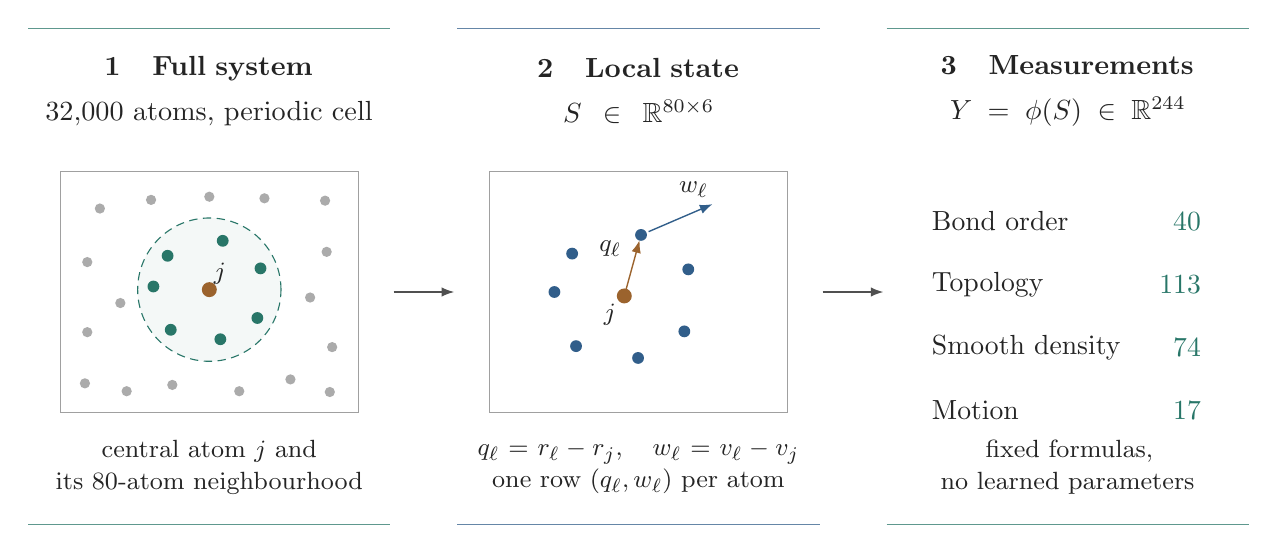
\begin{tikzpicture}[x=1cm,y=1cm]
  \foreach \left/\right/\tint in {.25/4.85/pcmGreen,5.70/10.30/pcmBlue,11.15/15.75/pcmGreen}{
    \draw[\tint!75,line width=.4pt] (\left,6.30) -- (\right,6.30);
    \draw[\tint!75,line width=.4pt] (\left,0) -- (\right,0);
  }
  \node[pcm/text,text width=4.40cm] at (2.55,5.50)
    {\textbf{1\quad Full system}\\[4pt]32,000 atoms, periodic cell};
  \node[pcm/text,text width=4.40cm] at (8.00,5.50)
    {\textbf{2\quad Local state}\\[4pt]$S\in\R^{80\times 6}$};
  \node[pcm/text,text width=4.40cm] at (13.45,5.50)
    {\textbf{3\quad Measurements}\\[4pt]$Y=\phi(S)\in\R^{244}$};
  \draw[pcm/arrow] (4.89,2.95) -- (5.66,2.95);
  \draw[pcm/arrow] (10.34,2.95) -- (11.11,2.95);

  % Full-system sketch: grey exterior, green selected atoms, highlighted centre.
  \draw[pcmRule,fill=white,line width=.4pt] (.66,1.42) rectangle (4.44,4.48);
  \fill[pcmGreen!5] (2.55,2.98) circle [radius=.91];
  \draw[pcmGreen,densely dashed,line width=.4pt] (2.55,2.98) circle [radius=.91];
  \foreach \xx/\yy in {.97/1.79,1.50/1.69,2.08/1.77,2.93/1.69,3.58/1.84,4.08/1.68,
    1.00/2.44,1.42/2.81,1.00/3.33,1.16/4.01,1.81/4.12,2.55/4.16,
    3.25/4.14,4.02/4.11,4.04/3.46,3.83/2.88,4.11/2.25}{
    \fill[pcmGray!48] (\xx,\yy) circle [radius=.065];
  }
  \foreach \xx/\yy in {2.02/3.41,2.72/3.60,3.20/3.25,3.16/2.62,
    2.69/2.35,2.06/2.47,1.84/3.02}{
    \fill[pcmGreen] (\xx,\yy) circle [radius=.075];
  }
  \fill[pcmAmber] (2.55,2.98) circle [radius=.095];
  \node[pcm/small,anchor=south west,text=pcmInk] at (2.60,3.04) {$j$};
  \node[pcm/small,text width=4.40cm] at (2.55,.72)
    {central atom $j$ and\\its 80-atom neighbourhood};

  % Local sketch, with a relative position and a relative velocity.
  \draw[pcmRule,fill=white,line width=.4pt] (6.11,1.42) rectangle (9.89,4.48);
  \foreach \xx/\yy in {7.1575/3.4375,8.0325/3.675,8.6325/3.2375,8.5825/2.45,7.995/2.1125,7.2075/2.2625,6.9325/2.95}{
    \fill[pcmBlue] (\xx,\yy) circle [radius=.075];
  }
  \fill[pcmAmber] (7.82,2.90) circle [radius=.095];
  \node[pcm/small,anchor=north east,text=pcmInk] at (7.72,2.80) {$j$};
  \draw[pcm/arrow,draw=pcmAmber,shorten >=2pt] (7.82,2.90) -- (8.0325,3.675);
  \node[pcm/small,text=pcmInk,anchor=east] at (7.79,3.50) {$q_\ell$};
  \draw[pcm/bluearrow,shorten <=3pt] (8.0325,3.675) -- (8.94,4.065);
  \node[pcm/small,text=pcmInk,anchor=south] at (8.70,4.14) {$w_\ell$};
  \node[pcm/small,text width=4.40cm] at (8.00,.72)
    {$q_\ell=r_\ell-r_j,\quad w_\ell=v_\ell-v_j$\\one row $(q_\ell,w_\ell)$ per atom};

  % Four fixed measurement groups.
  \foreach \yy/\labeltext/\number in {3.85/Bond order/40,3.05/Topology/113,2.25/Smooth density/74,1.45/Motion/17}{
    \node[pcm/text,anchor=west] at (11.72,\yy) {\labeltext};
    \node[pcm/text,anchor=east,text=pcmGreen] at (15.15,\yy) {\number};
  }
  \node[pcm/small,text width=4.40cm] at (13.45,.72) {fixed formulas,\\no learned parameters};
\end{tikzpicture}%
}

% Figure 2: the approach at a glance; simulation above, learned rollout below.
\newcommand{\PCMGlanceDiagram}{%
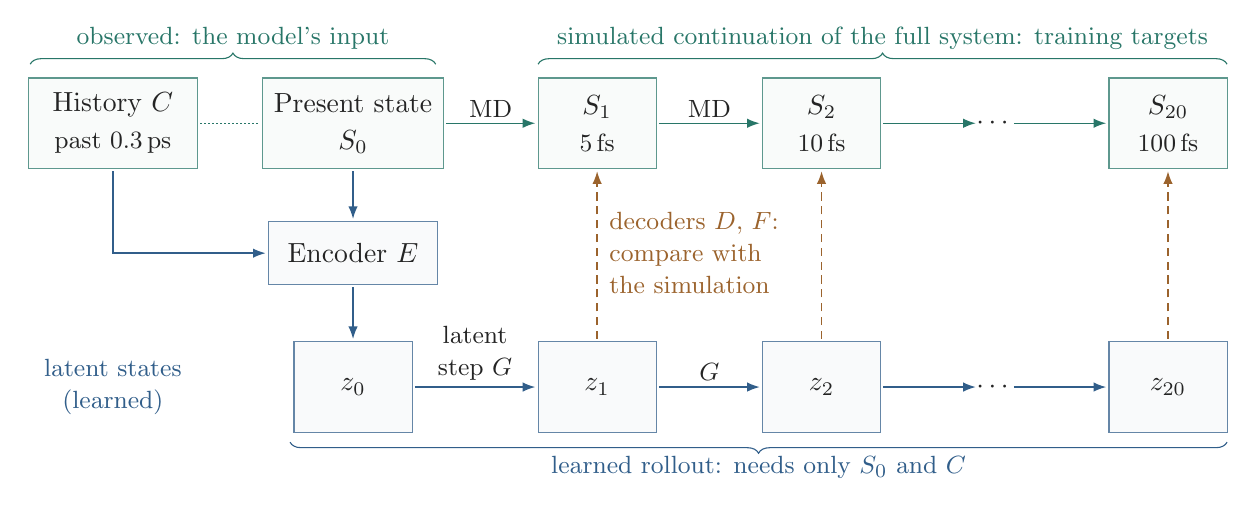
\begin{tikzpicture}[x=1cm,y=1cm]
  \tikzset{pcm/wide/.style={minimum width=2.15cm,minimum height=1.15cm},
           pcm/narrow/.style={minimum width=1.50cm,minimum height=1.15cm}}
  \node[pcm/physical,pcm/wide] (C)  at (1.10,4.10) {History $C$\\[1pt]{\fontsize{8.6}{10}\selectfont past 0.3\,ps}};
  \node[pcm/physical,pcm/wide] (S0) at (4.15,4.10) {Present state\\[1pt]$S_0$};
  \node[pcm/physical,pcm/narrow] (S1) at (7.25,4.10) {$S_1$\\[1pt]{\fontsize{8.6}{10}\selectfont 5\,fs}};
  \node[pcm/physical,pcm/narrow] (S2) at (10.10,4.10) {$S_2$\\[1pt]{\fontsize{8.6}{10}\selectfont 10\,fs}};
  \node[pcm/text] (Sd) at (12.30,4.10) {$\cdots$};
  \node[pcm/physical,pcm/narrow] (SK) at (14.50,4.10) {$S_{20}$\\[1pt]{\fontsize{8.6}{10}\selectfont 100\,fs}};
  \draw[pcmGreen,line width=.45pt,densely dotted] (C) -- (S0);
  \draw[pcm/greenarrow] (S0) -- node[pcm/small,above=2pt] {MD} (S1);
  \draw[pcm/greenarrow] (S1) -- node[pcm/small,above=2pt] {MD} (S2);
  \draw[pcm/greenarrow] (S2) -- (Sd);
  \draw[pcm/greenarrow] (Sd) -- (SK);
  \draw[pcm/brace,pcmGreen] (0.05,4.85) -- (5.20,4.85)
    node[midway,above=5pt,pcm/small,text=pcmGreen] {observed: the model's input};
  \draw[pcm/brace,pcmGreen] (6.50,4.85) -- (15.25,4.85)
    node[midway,above=5pt,pcm/small,text=pcmGreen] {simulated continuation of the full system: training targets};

  \node[pcm/model,minimum width=2.15cm,minimum height=.80cm] (E) at (4.15,2.45) {Encoder $E$};
  \draw[pcm/bluearrow] (S0) -- (E);
  \draw[pcm/bluearrow] (C.south) |- (E.west);

  \node[pcm/model,pcm/narrow] (z0) at (4.15,0.75) {$z_0$};
  \node[pcm/model,pcm/narrow] (z1) at (7.25,0.75) {$z_1$};
  \node[pcm/model,pcm/narrow] (z2) at (10.10,0.75) {$z_2$};
  \node[pcm/text] (zd) at (12.30,0.75) {$\cdots$};
  \node[pcm/model,pcm/narrow] (zK) at (14.50,0.75) {$z_{20}$};
  \draw[pcm/bluearrow] (E) -- (z0);
  \draw[pcm/bluearrow] (z0) -- node[pcm/small,above=2pt] {latent\\step $G$} (z1);
  \draw[pcm/bluearrow] (z1) -- node[pcm/small,above=2pt] {$G$} (z2);
  \draw[pcm/bluearrow] (z2) -- (zd);
  \draw[pcm/bluearrow] (zd) -- (zK);
  \foreach \k in {1,2,K}{
    \draw[pcm/amberarrow,densely dashed] (z\k.north) -- (S\k.south);
  }
  \node[pcm/small,anchor=west,align=left,text=pcmAmber] at (7.40,2.45)
    {decoders $D$, $F$:\\compare with\\the simulation};
  \node[pcm/small,text=pcmBlue] at (1.10,0.75) {latent states\\(learned)};
  \draw[pcm/brace,pcmBlue,decoration={mirror}] (3.35,0.05) -- (15.25,0.05)
    node[midway,below=5pt,pcm/small,text=pcmBlue] {learned rollout: needs only $S_0$ and $C$};
\end{tikzpicture}%
}

% Figure 3: identical reference paths, different responses.
\newcommand{\PCMFanDiagram}{%
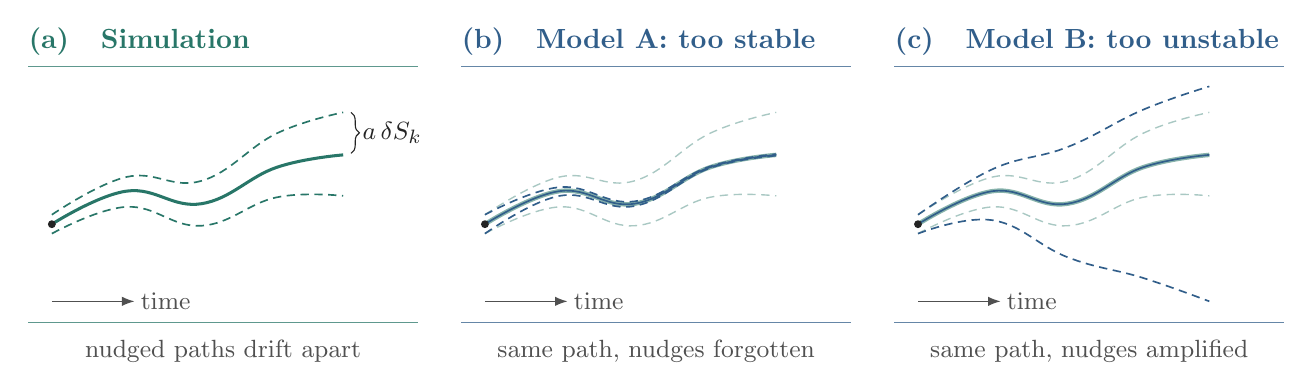
\begin{tikzpicture}[x=1cm,y=1cm]
  \foreach \dx/\tint/\title/\note in {
      0/pcmGreen/{(a)\quad Simulation}/{nudged paths drift apart},
      5.50/pcmBlue/{(b)\quad Model A: too stable}/{same path, nudges forgotten},
      11.00/pcmBlue/{(c)\quad Model B: too unstable}/{same path, nudges amplified}}{
    \begin{scope}[xshift=\dx cm]
      \node[pcm/head,text=\tint] at (0,3.72) {\title};
      \draw[\tint!75,line width=.4pt] (0,3.40) -- (4.95,3.40);
      \draw[\tint!75,line width=.4pt] (0,0.15) -- (4.95,0.15);
      \node[pcm/small,text=pcmGray] at (2.475,-0.22) {\note};
      \draw[pcm/arrow] (0.30,0.42) -- (1.35,0.42) node[right=2pt,pcm/tiny,text=pcmGray] {time};
    \end{scope}
  }
  % (a) the simulated reference path and two nudged paths.
  \draw[pcmGreen,line width=1.1pt] plot[smooth,tension=.7] coordinates
    {(.30,1.40) (1.25,1.82) (2.20,1.66) (3.15,2.12) (4.00,2.28)};
  \draw[pcmGreen,densely dashed,line width=.6pt] plot[smooth,tension=.7] coordinates
    {(.30,1.52) (1.25,2.00) (2.20,1.95) (3.15,2.55) (4.00,2.82)};
  \draw[pcmGreen,densely dashed,line width=.6pt] plot[smooth,tension=.7] coordinates
    {(.30,1.28) (1.25,1.62) (2.20,1.38) (3.15,1.74) (4.00,1.76)};
  \fill[pcmInk] (.30,1.40) circle [radius=.05];
  \draw[pcm/brace,pcmInk,decoration={amplitude=3pt}] (4.10,2.82) -- (4.10,2.30)
    node[midway,right=4pt,pcm/small] {$a\,\delta S_k$};
  % (b) and (c): the same path, with the simulated spread repeated in light green.
  \foreach \dx in {5.50,11.00}{
    \begin{scope}[xshift=\dx cm]
      \draw[pcmGreen!40,densely dashed,line width=.5pt] plot[smooth,tension=.7] coordinates
        {(.30,1.52) (1.25,2.00) (2.20,1.95) (3.15,2.55) (4.00,2.82)};
      \draw[pcmGreen!40,densely dashed,line width=.5pt] plot[smooth,tension=.7] coordinates
        {(.30,1.28) (1.25,1.62) (2.20,1.38) (3.15,1.74) (4.00,1.76)};
      \draw[pcmGreen!55,line width=1.6pt] plot[smooth,tension=.7] coordinates
        {(.30,1.40) (1.25,1.82) (2.20,1.66) (3.15,2.12) (4.00,2.28)};
      \draw[pcmBlue,line width=.6pt] plot[smooth,tension=.7] coordinates
        {(.30,1.40) (1.25,1.82) (2.20,1.66) (3.15,2.12) (4.00,2.28)};
      \fill[pcmInk] (.30,1.40) circle [radius=.05];
    \end{scope}
  }
  \begin{scope}[xshift=5.50cm]
    \draw[pcmBlue,densely dashed,line width=.6pt] plot[smooth,tension=.7] coordinates
      {(.30,1.52) (1.25,1.87) (2.20,1.69) (3.15,2.13) (4.00,2.29)};
    \draw[pcmBlue,densely dashed,line width=.6pt] plot[smooth,tension=.7] coordinates
      {(.30,1.28) (1.25,1.76) (2.20,1.63) (3.15,2.11) (4.00,2.27)};
  \end{scope}
  \begin{scope}[xshift=11.00cm]
    \draw[pcmBlue,densely dashed,line width=.6pt] plot[smooth,tension=.7] coordinates
      {(.30,1.52) (1.25,2.10) (2.20,2.38) (3.15,2.85) (4.00,3.15)};
    \draw[pcmBlue,densely dashed,line width=.6pt] plot[smooth,tension=.7] coordinates
      {(.30,1.28) (1.25,1.45) (2.20,0.98) (3.15,0.72) (4.00,0.42)};
  \end{scope}
\end{tikzpicture}%
}

% Figure 4: encoding should commute with time evolution, for states and for responses.
\newcommand{\PCMCommuteDiagram}{%
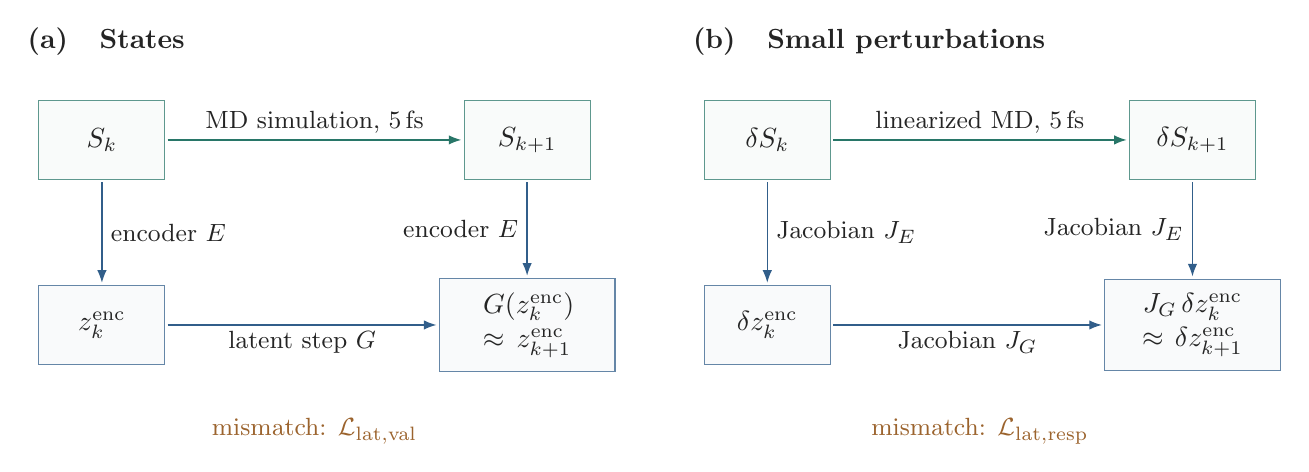
\begin{tikzpicture}[x=1cm,y=1cm]
  \tikzset{pcm/corner/.style={minimum width=1.60cm,minimum height=1.00cm}}
  \node[pcm/head] at (0,4.15) {(a)\quad States};
  \node[pcm/physical,pcm/corner] (aS)  at (0.95,2.90) {$S_k$};
  \node[pcm/physical,pcm/corner] (aS1) at (6.35,2.90) {$S_{k+1}$};
  \node[pcm/model,pcm/corner] (az) at (0.95,0.55) {$z^{\enc}_k$};
  \node[pcm/model,pcm/corner,text width=1.95cm] (az1) at (6.35,0.55)
    {$G(z^{\enc}_k)$\\$\approx z^{\enc}_{k+1}$};
  \draw[pcm/greenarrow] (aS) -- node[pcm/small,above=2pt] {MD simulation, 5\,fs} (aS1);
  \draw[pcm/bluearrow] (aS) -- node[pcm/small,right=3pt] {encoder $E$} (az);
  \draw[pcm/bluearrow] (aS1) -- node[pcm/small,left=3pt] {encoder $E$} (az1);
  \draw[pcm/bluearrow] (az) -- node[pcm/small,below=2pt] {latent step $G$} (az1);
  \node[pcm/small,text=pcmAmber] at (3.65,-0.80) {mismatch: $\mathcal L_{\rm lat,val}$};
  \begin{scope}[xshift=8.45cm]
    \node[pcm/head] at (0,4.15) {(b)\quad Small perturbations};
    \node[pcm/physical,pcm/corner] (bS)  at (0.95,2.90) {$\delta S_k$};
    \node[pcm/physical,pcm/corner] (bS1) at (6.35,2.90) {$\delta S_{k+1}$};
    \node[pcm/model,pcm/corner] (bz) at (0.95,0.55) {$\delta z^{\enc}_k$};
    \node[pcm/model,pcm/corner,text width=1.95cm] (bz1) at (6.35,0.55)
      {$J_G\,\delta z^{\enc}_k$\\$\approx\delta z^{\enc}_{k+1}$};
    \draw[pcm/greenarrow] (bS) -- node[pcm/small,above=2pt] {linearized MD, 5\,fs} (bS1);
    \draw[pcm/bluearrow] (bS) -- node[pcm/small,right=3pt] {Jacobian $J_E$} (bz);
    \draw[pcm/bluearrow] (bS1) -- node[pcm/small,left=3pt] {Jacobian $J_E$} (bz1);
    \draw[pcm/bluearrow] (bz) -- node[pcm/small,below=2pt] {Jacobian $J_G$} (bz1);
    \node[pcm/small,text=pcmAmber] at (3.65,-0.80) {mismatch: $\mathcal L_{\rm lat,resp}$};
  \end{scope}
\end{tikzpicture}%
}

% Figure 5: the Mori-Zwanzig decomposition of an observed quantity.
\newcommand{\PCMMoriDiagram}{%
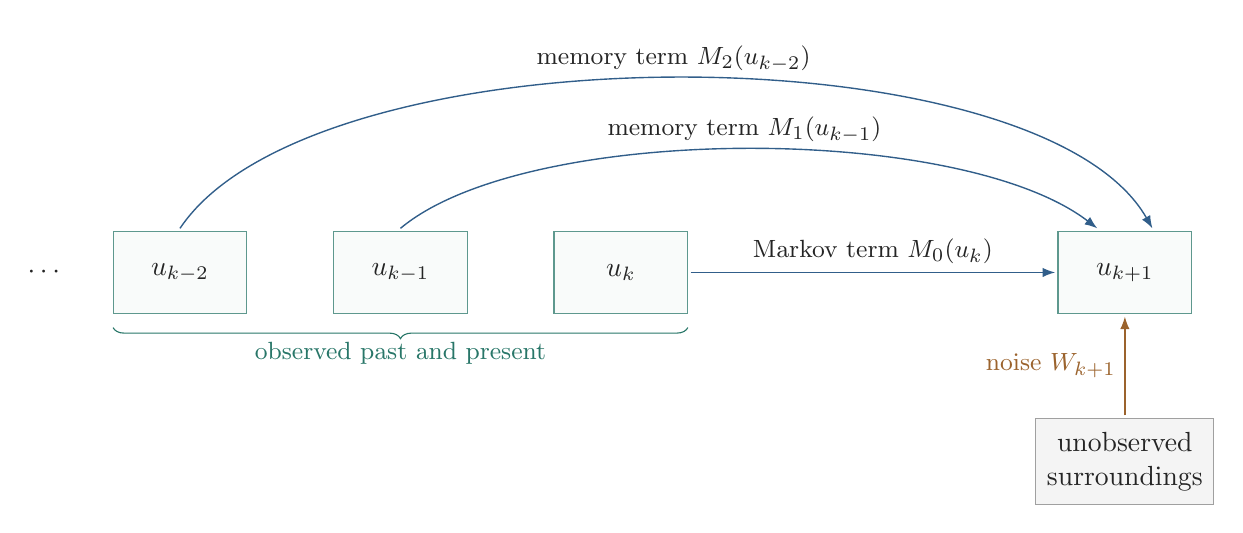
\begin{tikzpicture}[x=1cm,y=1cm]
  \tikzset{pcm/state/.style={minimum width=1.70cm,minimum height=1.05cm}}
  \node[pcm/text] (ud) at (0.40,1.00) {$\cdots$};
  \node[pcm/physical,pcm/state] (u2) at (2.10,1.00) {$u_{k-2}$};
  \node[pcm/physical,pcm/state] (u1) at (4.90,1.00) {$u_{k-1}$};
  \node[pcm/physical,pcm/state] (u0) at (7.70,1.00) {$u_{k}$};
  \node[pcm/physical,pcm/state] (un) at (14.10,1.00) {$u_{k+1}$};
  \draw[pcm/bluearrow] (u0) -- node[pcm/small,above=3pt] {Markov term $M_0(u_k)$} (un);
  % Nested arcs: the older observation reaches further up and lands further right.
  \draw[pcm/bluearrow] (u1.north) .. controls (6.50,2.90) and (12.00,2.90) .. ([xshift=-3.5mm]un.north)
    node[pos=.5,above=2pt,pcm/small] {memory term $M_1(u_{k-1})$};
  \draw[pcm/bluearrow] (u2.north) .. controls (3.80,4.10) and (13.00,4.10) .. ([xshift=3.5mm]un.north)
    node[pos=.5,above=2pt,pcm/small] {memory term $M_2(u_{k-2})$};
  \node[pcm/base,draw=pcmRule,fill=pcmGray!6] (env) at (14.10,-1.40) {unobserved\\surroundings};
  \draw[pcm/amberarrow] (env) -- node[pcm/small,left=3pt,text=pcmAmber] {noise $W_{k+1}$} (un);
  \draw[pcm/brace,pcmGreen,decoration={mirror}] (1.25,0.30) -- (8.55,0.30)
    node[midway,below=5pt,pcm/small,text=pcmGreen] {observed past and present};
\end{tikzpicture}%
}

\begin{document}
\setlength{\abovedisplayskip}{8pt plus 2pt minus 2pt}
\setlength{\belowdisplayskip}{8pt plus 2pt minus 2pt}
\setlength{\abovedisplayshortskip}{3pt plus 2pt}
\setlength{\belowdisplayshortskip}{6pt plus 2pt minus 2pt}
\maketitle\vspace{-2.6em}\thispagestyle{plain}

\begin{why}[The idea in five sentences]
\begin{enumerate}[leftmargin=1.5em]
\item We look at one atom's neighbourhood at a time: the 80 atoms nearest to it, with their
  positions and velocities.
\item A neural network learns to predict how this neighbourhood moves over the next 100\,fs, in
  steps of 5\,fs, from its present state and its recent past.
\item The network works in a learned internal representation, the \emph{latent state}, from which
  it reads out both the atomic motion and 244 standard structural measurements.
\item Besides the trajectory itself, the network learns how the trajectory responds to tiny changes
  of the initial positions or velocities, which we compute exactly from the simulation.
\item We then ask whether the latent state carries information about future crystallization beyond
  what the present structure already tells us.
\end{enumerate}
\end{why}

\section{What we want to find out}
\label{sec:question}

Crystallization of a supercooled liquid starts with small crystalline nuclei that
appear at particular places. We want to understand which local environments go
on to crystallize, and what distinguishes them from those that do not.

Standard structural descriptors are already strong predictors. In our nucleus
assay on supercooled Ni (Section~\ref{sec:findings}), a classifier that sees the
present and recent values of 244 such descriptors reaches an average precision
of about 0.7--0.8 for nuclei that appear 1--6\,ps later. Average precision (AP)
is the area under the precision--recall curve; a perfect classifier scores 1 and
a random guess scores 0.2 in this assay. For Ni it is also known that the
pre-structured liquid around a crystalline cluster, and not only the size of the
cluster, matters for the nucleation pathway~\cite{diazleines}. Structural
descriptors, however, mostly recognize order that is already present.

The question behind this work is whether the \emph{dynamics} of the liquid adds
information: how the local structure is moving, and how it would respond if it
were slightly disturbed. A direct way to capture such information is to learn a
model of the local dynamics and to use its internal state as a description of the
environment. A state that has to predict the next 100\,fs of motion and the
response to small perturbations must encode mechanical information---for
example, which directions of the local packing are soft and which are
stiff---in addition to the static structure.

Molecular dynamics (MD), the numerical integration of Newton's equations for all
atoms, is the teacher in this approach. The object of interest is the learned
local state and what it knows. The predicted trajectories serve two purposes:
they provide the training signal, and they test whether the learned state is
physically right.

\begin{why}[Why a local, learned model]
Interatomic forces in a metal are short-ranged, so over a short time an atom's
motion is determined mainly by its neighbourhood. The same physical law applies
to every atom at every time, so one local model can learn from many
neighbourhoods, and nucleation itself starts locally. A learned local model needs
only local information at prediction time: whatever it predicts correctly is
determined by local information, and its internal state can be compared directly
with the standard descriptors.
\end{why}

\section{What the model sees and what it learns from}
\label{sec:data}

\subsection{The local state}

Our data are MD simulations of supercooled liquid nickel. Each simulation cell is
periodic and contains 32,000 atoms, which interact through an embedded-atom
potential (a standard many-body interatomic potential for metals). The
simulations run at constant temperature and pressure, and snapshots are saved
every 0.1\,ps.

One example is defined by a saved snapshot and a central atom $j$. We number the
80 atoms nearest to $j$ by $\ell=1,\dots,80$, with $\ell=1$ the central atom
itself. With $r_\ell$ and $v_\ell$ the position and velocity of atom $\ell$ in the
simulation cell, its position and velocity relative to the central atom are
\begin{equation}
q_\ell=r_\ell-r_j,\qquad w_\ell=v_\ell-v_j .
\end{equation}
The \emph{local state} $S$ is the list of these 80 pairs,
$(q_1,w_1),\dots,(q_{80},w_{80})$, stored as an $80\times6$ array: one row per
atom, holding three position and three velocity components (the first row,
belonging to the central atom, is zero). Relative coordinates remove the absolute
position and the overall drift of the neighbourhood. The same 80 atoms are
followed in the past and in the future, so every row keeps referring to the same
atom. The model also receives the \emph{history} $C$: the local state of the same
80 atoms 0.1, 0.2 and 0.3\,ps before the present (Figure~\ref{fig:local}).

\begin{figure}[t]
\centering
\PlacePCMDiagram{\PCMLocalDiagram}
\caption{\textbf{From the full simulation to the local state and its measurements.}
The simulation moves all 32,000 atoms. The model works with the positions and velocities
of the 80 atoms nearest to a central atom $j$, relative to $j$; the fixed function $\phi$
turns this local state into 244 standard structural and motion measurements. The atom
drawings are schematic.}
\label{fig:local}
\end{figure}

\subsection{Short exact simulations as the teacher}
\label{sec:teacher}

For training targets, we restart the complete 32,000-atom system from the saved
snapshot and run it for 100\,fs at constant energy, saving the state every 5\,fs.
At constant energy the dynamics is deterministic: the same initial state always
gives the same trajectory. Each example thus has 20 simulated future local states
$S_1,\dots,S_{20}$ at elapsed times $\tau_k=k\cdot5$\,fs, with $S_0$ the present.
The simulation moves all atoms, including those outside the neighbourhood.

\begin{why}[Why short, dense, deterministic simulations]
Dense targets resolve the motion: in 5\,fs an atom moves only a few hundredths of
an \aa ngstr\"om, whereas the saved snapshots are 0.1\,ps apart. Deterministic
dynamics gives exactly defined responses to perturbations
(Section~\ref{sec:responses}). The continuation conserves energy, whereas the
original simulations hold the temperature fixed with a thermostat (a coupling to a
heat bath); over 100\,fs we accept this difference.

The 100-fs horizon also matches the time over which the neighbourhood mainly
determines its own motion. Sound in a liquid transition metal travels at about
4\,km/s, i.e.\ about 4\,\AA\ in 100\,fs, comparable to the ${\approx}\,6$\,\AA\
radius of the neighbourhood: influences from outside reach the inner atoms only
towards the end of the horizon, while the outermost atoms feel the surroundings
from the start. The history carries an imprint of these outside forces.
\end{why}

\subsection{Structural measurements}
\label{sec:measurements}

A fixed function $\phi$ maps a local state to 244 standard descriptors,
\begin{equation}
Y=\phi(S)\in\R^{244}.
\end{equation}
They are the kind of quantities physicists use to recognize local order, and they
fall into four groups.
\begin{itemize}[leftmargin=1.5em]
\item \emph{Bond order (40 numbers).} Steinhardt order parameters describe the
  symmetry of the directions from an atom to its 12 nearest neighbours, expanded in
  spherical harmonics of degree $l$. The magnitude $q_l$ measures how strongly these
  directions show $l$-fold symmetry; $q_6$, for example, is large in close-packed
  crystals. Averages $\bar q_l$ over neighbouring atoms reduce thermal noise; the
  invariants $w_l$ distinguish face-centred cubic, hexagonal close-packed and
  icosahedral arrangements; and the \emph{coherence} measures how similar the
  orientational order of neighbouring atoms is, which is high inside a crystal.
  All are computed for $l=2,4,6,8$.
\item \emph{Topology (113 numbers).} Persistent homology, a method of topological
  data analysis (TDA): place a ball on every atom and let all balls grow together.
  As the radius increases, separate balls merge into connected clusters, rings
  appear and are filled in, and enclosed cavities appear and are filled in. We
  record how many such features occur, at which radii they appear and disappear,
  how long they persist, and how many exist at fixed radii (the Betti numbers). In a
  crystal these events happen at a few well-defined radii; in a liquid they are
  spread out.
\item \emph{Smooth density (74 numbers).} The density of neighbours at four distances
  from the central atom, and, for every pair of these distances, the correlations
  between neighbour directions, expanded in Legendre polynomials of order 0--6. This
  is a smooth counterpart of bond order, similar to the widely used SOAP descriptor
  (smooth overlap of atomic positions).
\item \emph{Motion (17 numbers).} Statistics of the relative velocities: in three
  shells around the central atom, the mean radial velocity (are the neighbours
  approaching or receding?) and the spread of radial and tangential velocities; the
  rates at which the bond-order magnitudes for $l=2,4,6,8$ are changing under the
  present velocities; and a fit of the velocities by a uniform deformation of the
  neighbourhood (expansion, shear and rotation), together with the part of the
  motion that this fit leaves unexplained.
\end{itemize}
The density and motion groups (91 numbers, written $\phi_\sm$) are smooth
functions of the atomic coordinates. Bond order and topology change abruptly when
the set of nearest neighbours or the set of topological features changes;
derivatives are therefore used for the smooth group.

\begin{why}[Why the measurements are training targets]
$\phi$ enters training as a target: the model predicts the measurements from its
latent state. The latent state therefore has to acquire structural information
by learning the dynamics, and $\phi$ itself remains an independent reference for
comparison (Sections~\ref{sec:state} and~\ref{sec:findings}).
\end{why}

\subsection{Responses to small perturbations}
\label{sec:responses}

For each example we also store how the simulated future changes when the initial
condition is nudged. A nudge is a small random displacement of the 80 atoms,
applied either to their positions (root-mean-square size 0.01\,\AA) or to their
velocities (0.1\,\AA/ps); each example has one nudge of each kind. A nudge of
amplitude $a$ adds $a$ times the nudge direction to the initial state; let $S_k(a)$
be the local state that the simulation then reaches at time $\tau_k$. The
\emph{response}
\begin{equation}
\delta S_k=\frac{\partial S_k(a)}{\partial a}\bigg|_{a=0}
\end{equation}
is the change of the future local state per unit amplitude in the limit of a very
small nudge: a nudge of amplitude $a$ changes $S_k$ by approximately $a\,\delta S_k$.
We compute it exactly by integrating the equations of motion, linearized around the
simulated trajectory, alongside the trajectory itself. The nudge acts on the 80
atoms; all other atoms respond to it through the dynamics.

For a function $f$ of the state, $J_f(s)$ denotes its Jacobian at $s$ (the matrix
of its first derivatives), so that $J_f(s)\,d$ is the change of $f$ when $s$ moves
along the direction $d$. The responses of the smooth measurements then follow from
the chain rule, $\delta Y_{k,\sm}=J_{\phi_\sm}(S_k)\,\delta S_k$.

\section{The model}
\label{sec:model}

The model has four learned parts (Figure~\ref{fig:glance}): an encoder $E$, a
latent step $G$, an atomic decoder $D$ and a measurement decoder $F$. In one line,
\begin{equation}
(S_0,C)\xrightarrow{\;E\;}z_0\xrightarrow{\;G\;}z_1\xrightarrow{\;G\;}\cdots\xrightarrow{\;G\;}z_{20},
\qquad
\widehat S_k=S_0+D(z_k)-D(z_0),\qquad
\widehat Y_k=F(z_k),
\label{eq:model}
\end{equation}
where hats denote predictions. The input is the present local state $S_0$ and the
history $C$. From $z_0$ onwards, each step starts from the previous latent state,
with the history held fixed; we call the resulting sequence of predicted states a
\emph{rollout}. Table~\ref{tab:notation} collects the notation.

\begin{figure}[t]
\centering
\PlacePCMDiagram{\PCMGlanceDiagram}
\caption{\textbf{The approach at a glance.} Top: the observed input and the simulated
continuation, which provides the training targets. Bottom: the learned rollout. The encoder
$E$ maps the present state $S_0$ and the history $C$ to a latent state $z_0$; the latent
step $G$ advances it by 5\,fs at a time. At every step the atomic decoder $D$ and the
measurement decoder $F$ turn $z_k$ into predicted atoms $\widehat S_k$ and measurements
$\widehat Y_k$, which are compared with the simulation. The same picture applies to
responses: nudging $S_0$ changes every $z_k$, and the decoded changes are compared with the
simulated responses $\delta S_k$.}
\label{fig:glance}
\end{figure}

\begin{table}[ht]
\centering\small
\caption{Notation.}
\label{tab:notation}
\renewcommand{\arraystretch}{1.12}
\begin{tabularx}{\linewidth}{@{}>{\raggedright\arraybackslash}p{3.0cm} >{\raggedright\arraybackslash}X@{}}
\toprule
Symbol & Meaning\\
\midrule
$j$;\ $\ell=1,\dots,80$ & central atom; numbering of the atoms in its neighbourhood ($\ell=1$ is $j$)\\
$q_\ell$, $w_\ell$ & position and velocity of atom $\ell$ relative to the central atom\\
$S_k$ & local state at time $\tau_k=k\cdot5$\,fs: all $(q_\ell,w_\ell)$, an $80\times6$ array\\
$C$ & history: the local state 0.1, 0.2 and 0.3\,ps before the present\\
$Y_k=\phi(S_k)$ & the 244 fixed measurements; $\phi_\sm$ selects the 91 smooth ones\\
$z_k$ & latent state: eight three-dimensional vectors per atom\\
$E$, $G$, $D$, $F$ & encoder, latent step, atomic decoder, measurement decoder\\
$\widehat S_k$, $\widehat Y_k$ & predicted local state and measurements\\
$\delta S_k$, $\delta Y_k$ & responses: change of $S_k$, $Y_k$ per unit amplitude of a nudge of the initial state\\
$J_f(s)\,d$ & change of a function $f$ at $s$ along the direction $d$\\
\bottomrule
\end{tabularx}
\end{table}

\subsection{Encoder: the state of the neighbourhood}

$E$ maps the present state and its history to a latent state with eight
three-dimensional vectors per atom, $z\in\R^{80\times8\times3}$: one row of eight
vectors for every atom. At the start of training, two of these eight vectors are
the atom's relative position and velocity, and the other six are random
combinations of the two; training then shapes all eight. The encoder has two kinds
of layers. In the spatial layer, every atom combines its own vectors with the
relative positions and velocities of its neighbours within 6\,\AA, weighted by
learned functions of the interatomic distances. In the two attention layers, every
atom forms a weighted average of its own features at the present and at the three
past times, with weights computed from the features themselves.

\begin{why}[Why vectors for every atom]
The physics of the liquid has no preferred direction. The spatial layer builds each
output vector from relative positions and velocities, with weights that depend only
on distances and angles; rotating the input therefore rotates all latent vectors in
the same way (this property is called rotation equivariance). The model then needs
no data to learn rotations, and every atom carries vectors that can represent the
direction in which it moves. All 80 atoms are treated by the same rule, so
relabelling the input atoms relabels the output rows in the same way.
\end{why}

\begin{why}[Why the history]
The 80 atoms are part of a larger system: atoms outside the neighbourhood keep
pushing on them, so the present local state does not fully determine the future.
The recent motion of the tracked atoms carries an imprint of these outside forces.
The Mori--Zwanzig formalism (Section~\ref{sec:mz}) makes this precise: describing
a system through part of its variables produces a dependence on the past (memory)
and an unpredictable contribution from the rest (noise).
\end{why}

\subsection{Latent step: a learned integrator}

One step advances the latent state by $h=5$\,fs:
\begin{equation}
G(z)=z+\Delta_v(z)+\varepsilon\,\mathcal V(z).
\label{eq:step}
\end{equation}
The first increment, $\Delta_v(z)$, is the change of position under constant
velocity: the decoded velocity of each atom times 5\,fs, added to the latent
vectors through the same linear map that the encoder uses for positions. The second
term, $\mathcal V$, is a learned spatial layer of the same kind as in the encoder,
computed from the decoded relative positions and velocities of neighbouring atoms;
it plays the role of the forces. The fixed small factor $\varepsilon$ keeps each
step close to the identity.

\begin{why}[Why the step contains constant-velocity motion]
Over 5\,fs an atom moves almost in a straight line at its current velocity: forces
change the velocity only gradually. Constant-velocity motion is known exactly, so
the step contains it explicitly; it is also the first part of a standard MD time
step. The network then learns only the deviation caused by the interactions
between atoms. Keeping each step close to the identity keeps a 20-step rollout, and
its derivatives, well behaved. The history enters every step through the decoder
$D$, which attends to it.
\end{why}

\subsection{Decoders: atoms and measurements}

The atomic decoder $D$ maps a latent state to relative positions and velocities;
like the encoder, it attends to the history. The prediction is anchored at the
observed present, $\widehat S_k=S_0+D(z_k)-D(z_0)$: at $k=0$ it equals $S_0$
exactly, and for $k\ge1$ the network predicts the change since the present. The
measurement decoder $F$ maps a latent state to the 244 measurements, each
standardized to zero mean and unit variance over the training data. $F$ uses only
dot products between latent vectors, which stay the same when the whole
neighbourhood is rotated; its output is therefore rotation invariant, like $\phi$.

\begin{why}[Why the anchor]
The decoder reconstructs a state only approximately, and the changes we want to
predict are small: even after 100\,fs, assuming that nothing moves gives a
root-mean-square position error of only about 0.36\,\AA. A small reconstruction
error at time zero would be a large fraction of this signal; the anchor removes it.
\end{why}

\begin{why}[Why a learned measurement decoder]
$F$ serves two purposes. In training, fitting $F(z_k)$ to the measured $Y_k$ makes
the latent state carry structural information explicitly, at every time---the
information later read out for nucleation. And $F$ gives a prediction of future
structure whose derivatives exist for all 244 measurements. For evaluation, we also
apply $\phi$ to the predicted atoms, $\phi(\widehat S_k)$, and compare the two
predictions of the same measurements.
\end{why}

\section{Training: three kinds of supervision}
\label{sec:training}

All four parts are trained together on the simulated continuations, with three
kinds of supervision (Table~\ref{tab:losses}): values along the trajectory,
consistency between the parts, and responses to perturbations.

\begin{table}[ht]
\centering\small
\caption{Training losses. $z^{\enc}_k=E(S_k)$ is the encoding of a simulated state (with the
same fixed history); $z_k$ is the model's own rollout.}
\label{tab:losses}
\renewcommand{\arraystretch}{1.12}
\begin{tabularx}{\linewidth}{@{}l >{\raggedright\arraybackslash}p{5.2cm} >{\raggedright\arraybackslash}X@{}}
\toprule
Loss & Compares & Purpose\\
\midrule
\multicolumn{3}{@{}l}{\textit{Values along the trajectory}}\\
$\mathcal L_{\rm path}$ & predicted and simulated atoms, $\widehat S_k$ vs.\ $S_k$ & the forecast itself\\
$\mathcal L_{Y,0}$, $\mathcal L_{Y,+}$ & $F(z_k)$ vs.\ $Y_k$, now and in the future & keep structure in the latent state\\
$\mathcal L_{\Delta Y}$ & changes $\widehat Y_{k+1}-\widehat Y_k$ vs.\ $Y_{k+1}-Y_k$ & get the time evolution of structure right, as well as its level\\
\midrule
\multicolumn{3}{@{}l}{\textit{Consistency}}\\
$\mathcal L_{\rm kin}$ & successive displacements vs.\ integrated velocities & positions and velocities must agree\\
$\mathcal L_{\rm rec}$ & $D(z^{\enc}_k)$ vs.\ $S_k$ & the latent state holds the full atomic state\\
$\mathcal L_{\rm lat,val}$ & $G(z^{\enc}_0)$ vs.\ $z^{\enc}_1$ & encoding and stepping can be done in either order\\
\midrule
\multicolumn{3}{@{}l}{\textit{Responses}}\\
$\mathcal L_u$ & predicted and simulated atomic responses & correct sensitivity of the motion\\
$\mathcal L_R$ & predicted and simulated responses of the 91 smooth measurements & correct sensitivity of the structure\\
$\mathcal L_{\rm lat,resp}$ & one learned step applied to an encoded response vs.\ the next encoded response & the same for perturbations\\
\bottomrule
\end{tabularx}
\end{table}

The training objective is a weighted sum of these terms with fixed weights,
$\mathcal L=\sum_i\lambda_i\mathcal L_i$. Each term is first made dimensionless by
dividing it by a fixed scale computed from the training data---for example, the
error of constant-velocity prediction at each time for $\mathcal L_{\rm path}$, or
the typical size of the simulated response at each time for $\mathcal L_u$---so
that the terms can be added. Each training step uses rollouts of different
lengths, from a single step to all 20: long rollouts expose accumulated errors,
and short ones give cheap and stable updates.

The training set contains 320 starting snapshots from 28 independent simulations;
the test set contains 310 snapshots from 62 other simulations and is used only for
evaluation. Because the two sets come from different simulations, no test example
shares its history with a training example. All scales are computed from the
training data; each configuration is trained three times from different random
initializations and evaluated at the end of training.

\begin{why}[Why the consistency losses]
They impose physics and structure that the value losses leave open. Positions and
velocities are decoded separately, so $\mathcal L_{\rm kin}$ requires successive
displacements to match the integrated velocities, as they must. $\mathcal L_{\rm rec}$
requires that the full atomic state can be read back from any encoded state, which
gives the latent coordinates a physical meaning. $\mathcal L_{\rm lat,val}$ requires
that one learned step from the encoded present lands on the encoding of the
simulated next state (Figure~\ref{fig:commute}a), so that the rollout stays among
the states the encoder actually produces.
\end{why}

\section{Why train on derivatives?}
\label{sec:derivatives}

Response (derivative) supervision is the least standard part of the approach. Four
reasons motivate it.

\subsection{Responses describe the behaviour near the data}

The value losses compare the model with one simulated trajectory per example.
Many dynamical models reproduce that trajectory and still behave very differently
for nearby initial conditions (Figure~\ref{fig:fan}). The response $\delta S_k$
describes, to first order, this fan of nearby trajectories, and the response
losses compare the model's fan with the simulation's.

\begin{figure}[b]
\centering
\PlacePCMDiagram{\PCMFanDiagram}
\caption{\textbf{What responses add to values.} Each panel shows one coordinate of the local
state against time (schematic). All three panels share the same reference path (solid), so
value losses cannot tell the models apart. Dashed lines start from two slightly nudged
initial conditions; the light dashed lines in (b) and (c) repeat the simulated behaviour from
(a). Model A forgets the nudge, model B amplifies it. Response supervision matches the spread
of the dashed lines, which to first order is $a\,\delta S_k$. In a rollout, the model's own
small errors act like nudges, so the same property governs how its errors grow.}
\label{fig:fan}
\end{figure}

\subsection{The model's response governs its own error growth}

In a rollout, each step makes a small error, which the following steps treat as a
perturbation of their input. How such errors grow is set by the Jacobians of the
model---the same quantities that determine its response. A model that is too stable
forgets its initial condition and drifts towards an average prediction; one that is
too unstable amplifies its own errors. Matching the simulated responses calibrates
the growth of errors directly.

\subsection{More information per simulated example}

Each continuation provides one trajectory; each response adds a second, equally
detailed set of targets along it, for the cost of integrating the linearized
equations alongside the original ones. With 320 training snapshots, this matters.
Supervising derivatives as well as values is known to improve data efficiency and
generalization when fitting functions (Sobolev training, Section~\ref{sec:related}).

\subsection{Responses carry physical, causal information}

A response answers a what-if question: had these atoms been displaced slightly,
how would the neighbourhood have moved, and how would its structure have changed?
For short times the answer has a simple form. Write $X$ for the positions of all
atoms and $V$ for their velocities. Linearizing Newton's equations around the
trajectory gives, for a position nudge $\delta X_0$ and a velocity nudge
$\delta V_0$,
\begin{equation}
\delta X(\tau)\approx\delta X_0+\tau\,\delta V_0-\frac{\tau^2}{2m}\,H\,\delta X_0,
\label{eq:hessian}
\end{equation}
where $m$ is the atomic mass and $H$ is the Hessian of the potential energy (the
matrix of its second derivatives, i.e.\ the force constants) at the present
configuration. The approximation holds for times well below a vibrational period
(about 0.1--0.2\,ps). The short-time response to a position nudge therefore measures
the stiffness of the local packing along the nudged direction, information that
complements structural descriptors such as bond order. In glass-forming liquids, localized soft
vibrational modes are known to mark where structural rearrangements
occur~\cite{softmodes}; whether a comparable mechanical signal precedes
crystallization in Ni is one of the questions this representation is meant to help
answer. The measurement responses $\delta Y_\sm$ ask the question in structural
terms: how does a nudge change the local density correlations and motion
statistics over the following 100\,fs?

\subsection{How the derivatives enter training}

The model's own response is computed exactly by automatic differentiation, which
evaluates $J\,d$ for a program at a cost comparable to one extra evaluation. It is
propagated through the encoder and every step,
\begin{equation}
\delta z_0=J_E(S_0)\,\delta S_0,\qquad \delta z_{k+1}=J_G(z_k)\,\delta z_k,
\end{equation}
and then decoded into $\delta\widehat S_k$ and $\delta\widehat Y_{k,\sm}$. As in the
simulation, the nudge acts on the present state and the history stays fixed. The
response losses $\mathcal L_u$ and $\mathcal L_R$ compare the decoded responses with
the simulated ones and, like any other loss, are minimized with respect to the
network parameters.

Two further terms require that encoding and time evolution can be applied in
either order, for states and for small perturbations alike (Figure~\ref{fig:commute}).
We call the second one, $\mathcal L_{\rm lat,resp}$, \emph{latent transport}: it
carries a small perturbation along with the state. Both act on single 5-fs
transitions of the simulated path, so they supervise the step $G$ directly at any
intermediate time.

\begin{figure}[t]
\centering
\PlacePCMDiagram{\PCMCommuteDiagram}
\caption{\textbf{Encoding and time evolution in either order.} (a) Encoding the simulated
next state should give the same latent state as one learned step from the encoded present.
(b) The same for a small perturbation carried along with the state: the Jacobian of the
latent step, $J_G$, should map the encoded response at $\tau_k$ to the encoded response at
$\tau_{k+1}$. Here $\delta z^{\enc}_k=J_E(S_k)\,\delta S_k$, and both comparisons use the same
fixed history.}
\label{fig:commute}
\end{figure}

\subsection{What to expect}
\label{sec:expect}

The model sees the neighbourhood and its recent past, whereas the simulated
response also depends on the surrounding atoms. Moreover, the liquid is chaotic:
nearby trajectories separate exponentially fast, so perturbations grow and spread
with time. The best achievable local prediction of the response therefore becomes
less accurate as the horizon grows. We measure response error relative to the
prediction of zero response, which scores 1; values below 1 mean that part of the
response is predicted. The simulated responses belong to the constant-energy
continuation of the full system.

\section{The learned state and the fixed measurements}
\label{sec:state}

The encoder determines the model's \emph{state}: the object that the step $G$
advances in time. A good state for this role is
\begin{enumerate}[label=(\roman*),leftmargin=2em]
\item \emph{closed}: its future is determined by its present value, given the fixed history;
\item \emph{informative} about what we care about, here structure and its evolution;
\item \emph{differentiable}, with a well-defined behaviour under rotations, so that responses
  can be supervised.
\end{enumerate}
Table~\ref{tab:states} compares three candidates: the atoms alone, the measurements
$\phi$, and the learned latent state. The measurements are an excellent
description of structure; the learned latent state is designed to serve as the
state of the dynamics. Our current ideas combine the two.

\begin{table}[ht]
\centering\small
\caption{Three possible states for the dynamics.}
\label{tab:states}
\renewcommand{\arraystretch}{1.12}
\begin{tabularx}{\linewidth}{@{}>{\raggedright\arraybackslash}p{2.35cm}
  >{\raggedright\arraybackslash}X >{\raggedright\arraybackslash}X >{\raggedright\arraybackslash}X@{}}
\toprule
 & Atoms alone, $S$ & Measurements, $Y=\phi(S)$ & Learned latent, $z=E(S_0;C)$\\
\midrule
Contents & positions and velocities of the 80 atoms & 244 rotation-invariant summaries
  & the atoms (two channels), six learned vectors per atom, and the history\\
Closed? & partly: the surroundings act on the atoms, and the state has no room for what is inferred about them
  & partly: arrangements with the same $Y$ can have different futures
  & approached through the consistency losses\\
Responses & exact targets for every coordinate & for the 91 smooth components
  & exact, through $J_E$ and $J_G$\\
Predicted states & atomic configurations & values that must be checked for realizability
  & decoded to atomic configurations\\
Structure explicit? & through $\phi$ & yes, by construction & as far as learned, through $F$\\
\bottomrule
\end{tabularx}
\end{table}

\subsection{The learned latent as the state}

The latent state contains the atomic state (two of its channels) and six additional
vector channels per atom, which can carry information about the surroundings and
the past. The training losses push it towards closure (consistency), structural
content ($F$) and correct sensitivity (responses), and it is differentiable by
construction. Its structural information has to be learned from the data: 320
training snapshots, compared with the decades of physical insight built into $\phi$.

\subsection{The measurements as a description}

$\phi$ condenses the structure into interpretable numbers that already predict
nucleation well. As a state for the dynamics, it has three properties to account
for. It is rotation invariant and assigns the same values to many different atomic
arrangements, so the future of $Y$ depends on more than its present value: in terms
of $Y$ alone the dynamics is stochastic, and the randomness comes from everything
that $\phi$ summarizes. Predicted values of $Y$ must be checked for
\emph{realizability}, i.e.\ whether some arrangement of atoms produces them. And
derivatives are available for the 91 smooth measurements. Section~\ref{sec:mz}
gives the natural framework for dynamics in such variables.

\subsection{Ideas for combining them}
\label{sec:ideas}

\begin{enumerate}[label=(\alph*),leftmargin=2em]
\item \emph{$\phi$ as an additional encoder input}, $z_0=E(S_0,\phi(S_0);C)$: the latent state
  starts from the known structural information, and the dynamics and responses stay in the
  atomic state.
\item \emph{The structural part of the encoder learned from all saved snapshots}: $\phi$ can be
  computed on every saved snapshot of every simulation, which provides far more examples than
  the 320 teacher snapshots; the dynamics and responses are learned from the teacher
  simulations.
\item \emph{A stochastic model for the dynamics of $\phi$}, or of a compressed version of it, with
  responses supervised for the smooth measurements and generated values checked for
  realizability.
\end{enumerate}
In (a) and (b) the latent state contains the information in $\phi$ by
construction. The test then becomes whether it adds information beyond $\phi$: we
compare a classifier that receives $\phi$ alone with one that receives $\phi$
together with the learned features.

\section{What we test, and what we have found so far}
\label{sec:findings}

We compare four configurations of the training objective, each trained three
times. All share the atomic, consistency and response losses of
Section~\ref{sec:training}; they differ in the measurement terms and in how many
5-fs transitions the latent transport loss $\mathcal L_{\rm lat,resp}$ covers
(Table~\ref{tab:configs}).

\begin{table}[ht]
\centering\small
\caption{The four configurations.}
\label{tab:configs}
\renewcommand{\arraystretch}{1.12}
\begin{tabularx}{\linewidth}{@{}>{\raggedright\arraybackslash}p{3.0cm}
  >{\raggedright\arraybackslash}p{3.6cm} >{\raggedright\arraybackslash}p{2.7cm} >{\raggedright\arraybackslash}X@{}}
\toprule
Configuration & Measurement terms & Latent transport & Question\\
\midrule
Present measurements & present values, $\mathcal L_{Y,0}$ & first transition
  & are dynamics plus present structure enough?\\
Future measurements & all values and changes, $\mathcal L_{Y,0}$, $\mathcal L_{Y,+}$, $\mathcal L_{\Delta Y}$
  & first transition & does supervising how structure evolves help?\\
Measurement responses & as above, plus $\mathcal L_R$ & first transition
  & does structural sensitivity help?\\
Multitransition transport & as future measurements & four per training step, cycling through all twenty
  & does more latent consistency help?\\
\bottomrule
\end{tabularx}
\end{table}

We evaluate atomic accuracy against two simple predictions (no motion; constant
velocity), response error relative to predicting zero response, the accuracy of
the decoded measurements, and nucleus prediction. For nucleus prediction, a
separately trained classifier receives features of the latent state, with the
network itself kept fixed, and predicts whether the central atom will be among the
first atoms of a crystalline nucleus---a connected crystalline cluster of at least
64 atoms that persists for at least 1.5\,ps---appearing 1, 3 or 6\,ps later. Each
nucleus contributes four of its first atoms and sixteen other atoms from the same
snapshot, so 20\% of the examples are positive. We report AP together with the log
loss (the negative log-probability given to the correct outcome) and the Brier
score (the mean squared difference between predicted probability and outcome),
which reward well-calibrated probabilities. AP serves only for evaluation; the
nucleus labels enter only the separately trained classifier. Intervals below are
95\% intervals for differences, obtained by resampling whole simulations. The main
findings so far:
\begin{itemize}[leftmargin=1.5em]
\item \emph{Response supervision improves short-time prediction.} In a comparison of a
  simpler model without history, adding atomic response supervision reduced the 100-fs
  position error by 13\%, and adding latent transport reduced it by a further 4\%. The
  response error, relative to zero response, fell from 1.01 to 0.56 at 50\,fs, and from
  2.03 to 0.97 at 100\,fs.
\item \emph{Measurement responses help the latent state.} Compared with the
  future-measurement configuration, nucleus AP from latent features along the predicted
  path rises by 0.06/0.02/0.04 at 1/3/6-ps lead times (intervals exclude zero), and the
  100-fs errors of the measurement decoder fall in all four groups (bond order, for
  example, from 1.01 to 0.64 in standardized units).
\item \emph{The latent state does not yet beat the measurements.} Latent features reach
  AP 0.56/0.51/0.43, against 0.80/0.81/0.72 for the measured history; adding the latent
  features to the measured history changes AP by at most $+0.01$, with intervals that
  include zero.
\item \emph{Responses at 100\,fs remain hard.} Measurement-response supervision lowers
  the smooth-measurement response error from 2.34 to 0.99 times the zero-response
  error: it removes excessive sensitivity, but does not yet predict the 100-fs response
  well. Atomic responses at 100\,fs stay at 0.77--0.79 times the zero-response error,
  similar to the same model trained without measurement terms (0.76).
\item \emph{Structure generalizes poorly from 320 snapshots.} With present measurements
  only, the measurement decoder's training loss is about 0.05, while its test error is
  about 1.65.
\item \emph{Multitransition transport} improves 100-fs velocity prediction but weakens
  the nucleus readouts.
\end{itemize}

\subsection*{Questions for discussion}
\begin{enumerate}[leftmargin=1.5em]
\item Structure should not have to be rediscovered from 320 snapshots: which of the
  ideas in Section~\ref{sec:ideas} should we try first?
\item Response supervision clearly helps at short times, but the 100-fs responses
  remain near the zero-response level. Is the limit the horizon, the locality of the
  input, or the amount of data?
\item The central question---whether the dynamics adds information about
  crystallization beyond $\phi$---is still open: so far the learned state adds at most
  a small, non-significant amount to the measured history.
\end{enumerate}

\section{Next step: a Mori--Zwanzig model of the local dynamics}
\label{sec:mz}

The neighbourhood is part of a much larger system. The Mori--Zwanzig
formalism~\cite{mori,zwanzig} rewrites the exact dynamics of a full system as an
equation for a chosen set of observed variables alone, with additional terms that
account for everything unobserved. We plan to use it as the framework for modelling
the local dynamics.

Let $\Gamma_k$ be the complete state of the simulation (positions and velocities of
all 32,000 atoms) at time $\tau_k$; one MD step of 5\,fs maps $\Gamma_k$ to
$\Gamma_{k+1}$. Let $u_k=u(\Gamma_k)$ be the variables we observe: the local state
$S_k$, its latent encoding $z_k$, or the measurements $Y_k$. Let $\mathcal P$ be the
operation that averages a quantity over all complete states sharing the same observed
value---over all arrangements of the surrounding atoms compatible with what we see,
weighted by how likely they are in the liquid. With these definitions, the observed
variables obey exactly
\begin{equation}
\boxed{u_{k+1}=M_0(u_k)+\sum_{l=1}^{k}M_l(u_{k-l})+W_{k+1}.}
\label{eq:mz}
\end{equation}
The three terms have a direct meaning (Figure~\ref{fig:mz}).
\begin{itemize}[leftmargin=1.5em]
\item \emph{Markov term} $M_0(u_k)$: the average next value given the present one, i.e.\ the best
  prediction that uses the present alone. (A Markov process is one whose future depends only on
  its present.)
\item \emph{Memory terms} $M_l(u_{k-l})$, $l\ge1$: corrections from observations $l$ steps in the
  past. The surroundings were shaped by earlier local states, and this influence returns later;
  for example, outer atoms pushed by the neighbourhood push back after a delay.
\item \emph{Noise term} $W_{k+1}$: the contribution of the unobserved part of the initial state.
  Its average vanishes for every observed initial value, $\mathcal P W_{k+1}=0$: it is the part of
  the future that the observations cannot predict.
\end{itemize}
Equation~\eqref{eq:mz} is exact; approximations enter through the choice of the
observed variables $u$, the number of past steps kept in the memory, and the model
of the noise. The better $u$ captures the relevant, slowly changing information, the
shorter the memory and the smaller the noise; a closed state in the sense of
Section~\ref{sec:state} is one for which both vanish. In continuous time the same
structure is the generalized Langevin equation,
$\dot u(t)=M(u(t))+\int_0^t K\big(u(t-s),s\big)\,\mathrm ds+F(t)$, with memory kernel
$K$ and noise $F(t)$.

\begin{figure}[t]
\centering
\PlacePCMDiagram{\PCMMoriDiagram}
\caption{\textbf{The Mori--Zwanzig decomposition in our notation.} The next observed value
$u_{k+1}$ (local state, latent state or measurements) is the sum of a Markov term that
depends on the present observation, memory terms that depend on past observations, and a
noise term that comes from the unobserved surroundings.}
\label{fig:mz}
\end{figure}

The current model already contains two of the three terms. The latent step $G$
plays the role of the Markov term in latent coordinates. Memory enters through the
attention to the history $C$, which covers the observed past before the forecast,
and through the six additional latent channels, which carry information forward
during the rollout; adding hidden variables that are carried along with the state
is a standard way to represent memory. The rollout itself is a single prediction,
an estimate of the average over the noise. We plan to make the structure explicit:
\begin{enumerate}[label=(\roman*),leftmargin=2em]
\item choose the observed variables $u$ and learn the Markov and memory terms, with a
  memory length determined from the data, for example from how quickly the memory terms
  decay with the lag $l$;
\item model the noise term $W$ as a random process, so that the model predicts a
  distribution of futures;
\item use the relations between the terms. When the average $\mathcal P$ is replaced by its
  best linear approximation in a liquid in equilibrium (Mori's linear version), the memory
  kernel equals the time correlation of the noise, normalized by the variance of $u$ (the
  second fluctuation--dissipation theorem). Memory and noise then describe the same
  unobserved surroundings and can be learned consistently. The responses $\delta S_k$ add
  information about how the future depends on the observed state.
\end{enumerate}

\section{Related work}
\label{sec:related}

\subsection{Learning effective dynamics in a latent space}

Vlachas et al.~\cite{led} learn the dynamics of a high-dimensional system in a
low-dimensional latent space (LED). An autoencoder---an encoder--decoder pair trained
so that $D(E(S))\approx S$---provides the maps between the two, $z=E(S)$ and
$\widehat S=D(z)$. A recurrent neural network advances the latent state while
carrying an internal memory $h_k$ of the latent states it has seen:
\begin{equation}
(z_{k+1},h_{k+1})=G(z_k,h_k).
\end{equation}
Both maps can be probabilistic: mixture density networks output the parameters of a
mixture of Gaussian distributions, giving a distribution of next latent states and
of reconstructed full states. The learned latent dynamics can alternate with short
runs of the full simulation, and the applications range from chemistry to fluid
mechanics. In our terms, LED has the same encoder--step--decoder structure; its
recurrent memory corresponds to our history attention and extra latent channels,
and its probabilistic transition to the noise term of Section~\ref{sec:mz}. Our model
adds response supervision and an atom-resolved latent state that rotates with the
input.

\subsection{Data-driven Mori--Zwanzig models}

Lin and Lu~\cite{linlu} derive the discrete-time Mori--Zwanzig equation
\eqref{eq:mz} from the Koopman operator, which maps any function of the complete
state to its value one time step later, and turn it into a practical model. They
keep a finite number $L$ of past steps and approximate each Markov and memory term
by a combination of chosen functions $\psi_i$ of the past observations,
\begin{equation}
u_{k+1}\approx\sum_{l=0}^{L}\sum_i c_{l,i}\,\psi_i(u_{k-l})+W_{k+1},
\end{equation}
with coefficients $c_{l,i}$ fitted by least squares on simulated trajectories (a
``Wiener projection''). The result is a NARMAX model: a nonlinear autoregression on
past observations, with a moving-average model of the noise. They demonstrate it on
the Kuramoto--Sivashinsky equation and on a viscous Burgers equation with random
forcing. In our notation, $u$ can be the local state $S$, the latent state $z$ or the
measurements $Y$, and the history $C$ supplies past observations. This is the most
direct template for the plan of Section~\ref{sec:mz}.

\subsection{Sobolev training}

To fit a model $f_\theta$ to a target function $f$, Czarnecki et
al.~\cite{sobolev} match derivatives as well as values:
\begin{equation}
\sum_x\Big[\ell\big(f_\theta(x),f(x)\big)+\ell\big(J_{f_\theta}(x),J_f(x)\big)\Big],
\end{equation}
where $\ell$ is a loss such as the squared error. When full Jacobians are too large,
they match derivatives along random directions $d$, $J_{f_\theta}(x)\,d\approx J_f(x)\,d$.
They report better data efficiency and generalization than with values alone. In
our notation, the target function is the map from the present local state to a
future one, $S_0\mapsto S_k$. The path loss matches its values; the response losses
match its derivatives along random nudge directions, $\delta\widehat S_k\approx\delta S_k$.
Our response supervision is therefore Sobolev training of the rollout along random
directions.

\begin{thebibliography}{9}
\bibitem{diazleines} G.~D\'iaz Leines and J.~Rogal, \emph{Maximum likelihood analysis of
  reaction coordinates during solidification in Ni}, arXiv:1810.04782 (2018).
\bibitem{mori} H.~Mori, \emph{Transport, collective motion, and Brownian motion}, Progress of
  Theoretical Physics~33, 423--455 (1965).
\bibitem{zwanzig} R.~Zwanzig, \emph{Nonequilibrium Statistical Mechanics}, Oxford University
  Press (2001).
\bibitem{softmodes} A.~Widmer-Cooper, H.~Perry, P.~Harrowell and D.~R.~Reichman,
  \emph{Irreversible reorganization in a supercooled liquid originates from localized soft
  modes}, Nature Physics~4, 711--715 (2008).
\bibitem{led} P.~R. Vlachas, G.~Arampatzis, C.~Uhler and P.~Koumoutsakos, \emph{Multiscale
  simulations of complex systems by learning their effective dynamics}, Nature Machine
  Intelligence~4, 359--366 (2022).
\bibitem{linlu} K.~K. Lin and F.~Lu, \emph{Data-driven model reduction, Wiener projections, and
  the Koopman--Mori--Zwanzig formalism}, Journal of Computational Physics~424, 109864 (2021).
\bibitem{sobolev} W.~M. Czarnecki, S.~Osindero, M.~Jaderberg, G.~\'Swirszcz and R.~Pascanu,
  \emph{Sobolev training for neural networks}, Advances in Neural Information Processing
  Systems~30 (2017).
\end{thebibliography}

\end{document}
